\documentclass[runningheads]{llncs}

\usepackage{graphicx}
\usepackage[english]{babel}
\usepackage{textcomp}

\graphicspath{{tavaeva/}}

\begin{document}

\title{A Cost Minimizing at Laser Cutting of Sheet Parts on CNC Machines}

\author{
  Tavaeva A.F. \inst{1}
  \and
  Petunin A.A. \inst{2,3}
  \and
  Kurennov D.V. \inst{2}
  \and Krotov V.I. \inst{4}
}

\institute{
  Production association ``Urals Optical and Mechanical Plant'', Yekaterinburg, Russia \url{http://www.uomz.ru/}
  \and
  Ural Federal University, Yekaterinburg, Russia \url{https://urfu.ru/}
  \and
  Institute of Mathematics and Mechanics, UBr RAS, Yekaterinburg, Russia \url{https://www.imm.uran.ru/}
  \and
  Joint-Stock Company ``Technocomproject'', Yekaterinburg, Russia
}
\maketitle              % typeset the header of the contribution

\begin{abstract}
The problem of cost minimizing at laser cutting of sheet parts on CNC machines is considered.
As an objective function the cost function of cutting process is used.
The model of exact cost function calculation is presented
depending on the number of frames in the NC program.
In order to solve the optimization problem the special cutting techniques are used.
There are multi-contour and multi-segment cutting techniques.
In this paper the special cutting techniques for common geometrical types of
contours widely used in blank production of engineering plant are presented.
The results of the computational experiment
which show a statistically significant improvement
of the objective function value compared
with using the standard cutting techniques are presented.

\keywords{CNC laser cutting machines \and thermal cutting \and tool path optimization \and cost of cutting process \and cutting techniques}
\end{abstract}

\section{Introduction}

Recently the CNC sheet cutting machines are widely used in blank production of engineering plant.
In particular such machines include thermal cutting machines (laser, flame and plasma cutting).
The CNC thermal cutting machines are worked by NC programs.
During development of NC program the some features and restrictions are arisen.

Before cutting of part contour the piercings must be selected (Fig. \ref{elements}).
Piercings are operations where the laser cutting tool initiates the material.
Piercings is selected according to the material type, its thickness and cutting parameters.
In order to avoid material beading and part deformation the piercings must be selected by some distance from contour.

\begin{figure}
  \begin{center}
  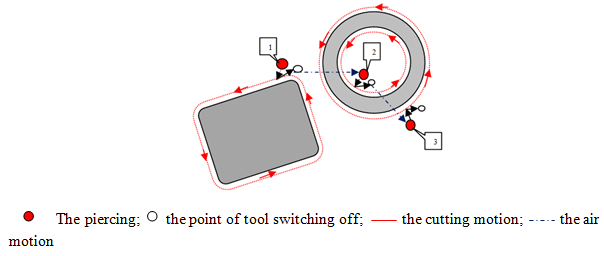
\includegraphics[width=0.9\textwidth]{elements.png}
  \caption{Cutting scheme example of two parts using standard cutting technique}
  \label{elements}
  \end{center}
\end{figure}

\section{Exact calculation of cost function $F_{cost}$ in cutting sheet material at CNC laser $CO_2$ machine}

\subsection{Model of basic cost parameters  $C_{on}, C_{off}, C_{pt}$ calculation}

The most important economic characteristic of the developed NC program quality is the cost $F_{cost}$
of cutting parts at CNC machine.
$F_{cost}$ includes the costs of electricity and expendable materials,
maintenance of a CNC machine and other operating costs incurred during cutting.
The problem of exact calculation of cost function $F_{cost}$
in optimizing of cutting tool route related with search of adequate value  $F_{cost}$,
which calculation depends on basic parameters  $C_{on}, C_{off}, C_{pt}$.

\subsection{Calculation of cutting tool speed $V_{on}$
and correction coefficient depending on the complexity of
part contours by example of the CNC laser cutting machine ByStar 3015}

The inaccuracy of the actual cutting time and cost calculation is due to the fact that $V_{on}$,
which is programmed as constant value in NC program,
is actually varied by various technological factors.
It was found that increasing of frames numbers in NC program
for various sets of parts,
which have the same total perimeter of the contours,
the actual $V_{on}$ is decreased [9,10].
The reasons why NC program can contain a large numbers of frames
is mainly due to the contours of complex geometry (for example, splines)
when converting from CAD systems to a CAM
are divided into a large numbers of geometric primitives
due to the difference of geometric file formats
(for example, on segments of straight lines and circular arcs),
i.e. approximated by simple geometric primitives.
The difference in formats is due to the fact that
almost all CNC systems are equipped with only linear and circular interpolators.
As a rule the approximation of a complex geometry reduces to a linear approximation.

\begin{figure}
  \begin{center}
  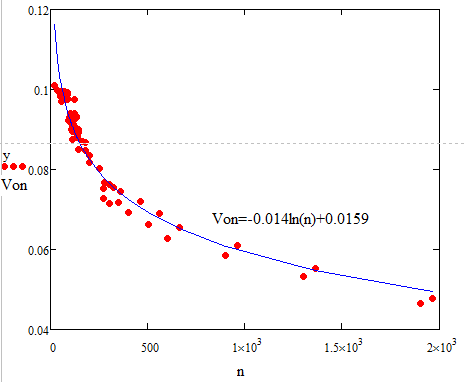
\includegraphics[width=0.77\textwidth]{plot.png}
  \caption{Change of the real cutting tool speed for Amg3M, $\Delta=1$ mm}
  \label{plot}
  \end{center}
\end{figure}


\section{Special cutting techniques used during optimization of cutting tool route}

\subsection{Classification of special cutting techniques}

The special cutting techniques used during minimization of basic objective function are classified into three classes [13]:

\begin{figure}
  \begin{center}
  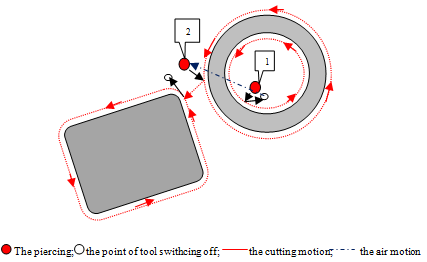
\includegraphics[width=0.9\textwidth]{chain.png}
  \caption{Cutting scheme example of two parts using ``chained'' cutting technique}
  \label{chain}
  \end{center}
\end{figure}

\begin{figure}
  \begin{center}
  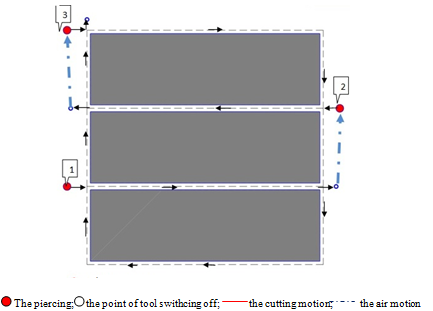
\includegraphics[width=0.9\textwidth]{common.png}
  \caption{Cutting scheme example of ``chained'' cutting technique}
  \label{common}
  \end{center}
\end{figure}

\begin{figure}
  \begin{center}
  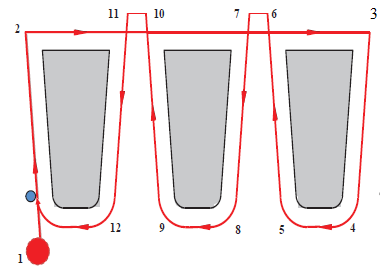
\includegraphics[width=0.6\textwidth]{snake.png}
  \caption{Cutting scheme example of snake cutting}
  \label{snake}
  \end{center}
\end{figure}

\subsection{Classification of special cutting techniques for circle and polygon parts}

The one method of cutting time and cost minimization is application of special cutting techniques.

In engineering industry the geometrical forms of most parts are polygon and circle.
This paper considers the special cutting techniques for polygons and circles parts.
The special cutting techniques use more complexity algorithm in contrast to standard cutting technique.

\begin{figure}
  \begin{center}
  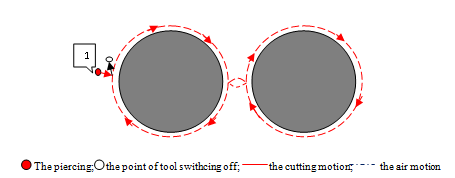
\includegraphics[width=0.9\textwidth]{8.png}
  \caption{Cutting scheme example of two parts using special cutting}
  \label{8}
  \end{center}
\end{figure}

\begin{figure}
  \begin{center}
  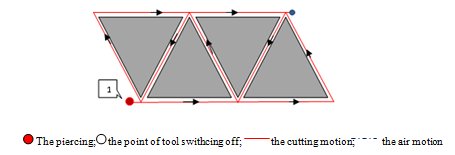
\includegraphics[width=0.9\textwidth]{tri.png}
  \caption{Cutting scheme example of four triangle parts using special cutting techniques}
  \label{tri}
  \end{center}
\end{figure}

\section{Computational experiments}

\begin{figure}
  \begin{center}
  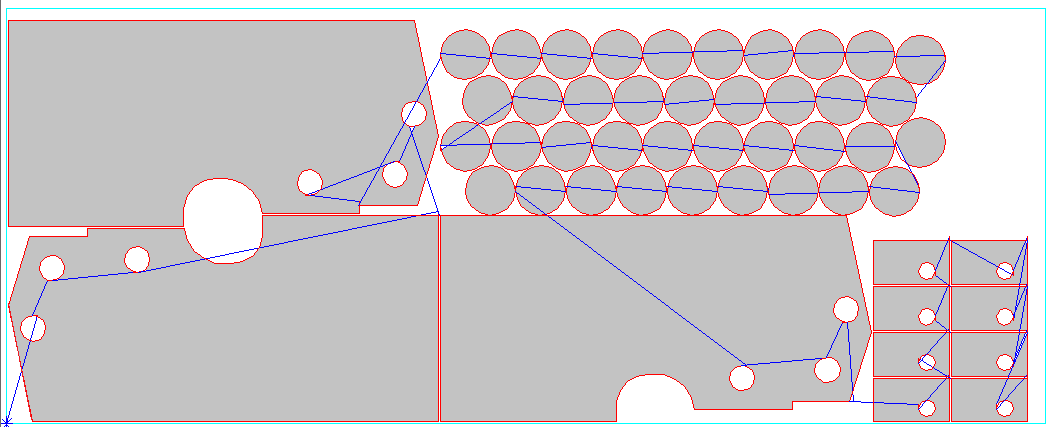
\includegraphics[width=0.9\textwidth]{std.png}
  \caption{Cutting scheme example of parts using standard cutting technique}
  \label{std}
  \end{center}
\end{figure}

\begin{figure}
  \begin{center}
  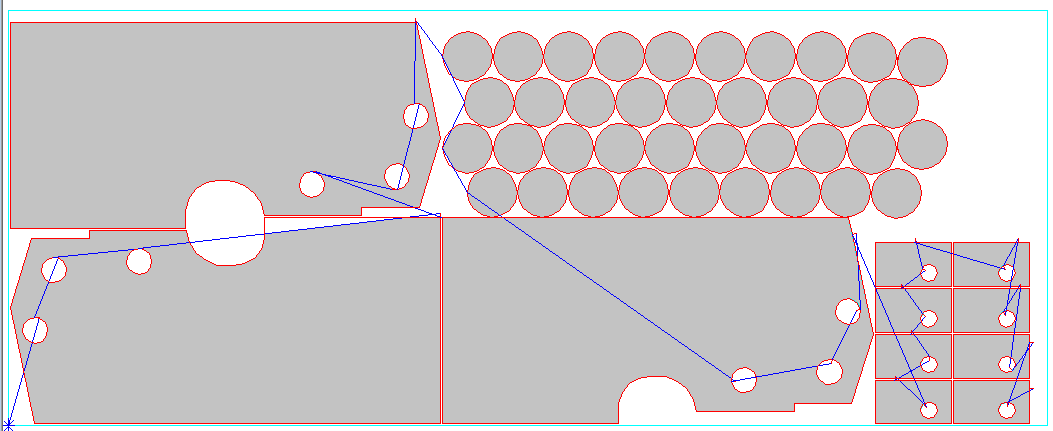
\includegraphics[width=0.9\textwidth]{special.png}
  \caption{Cutting scheme example of parts using special cutting technique}
  \label{special}
  \end{center}
\end{figure}

\begin{figure}
  \begin{center}
  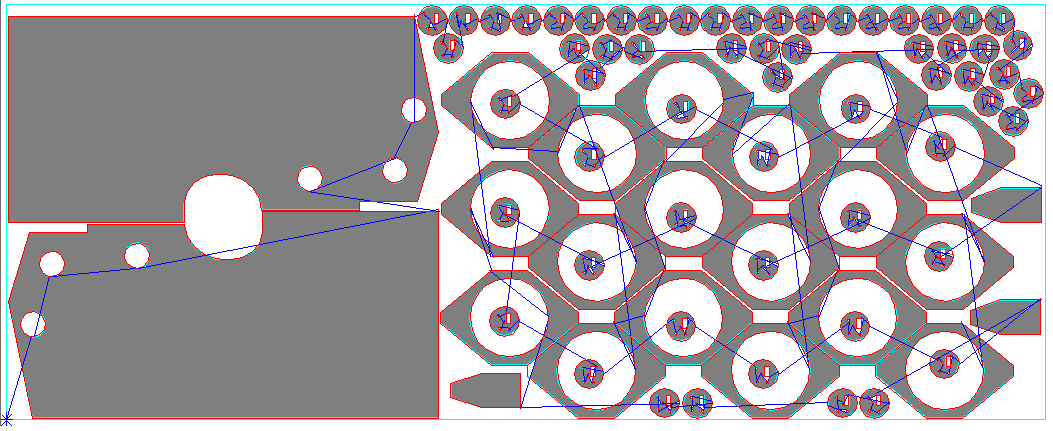
\includegraphics[width=0.9\textwidth]{spec-a.png}
  \caption{Cutting scheme example of parts using special cutting technique}
  \label{spec-a}
  \end{center}
\end{figure}

\begin{figure}
  \begin{center}
  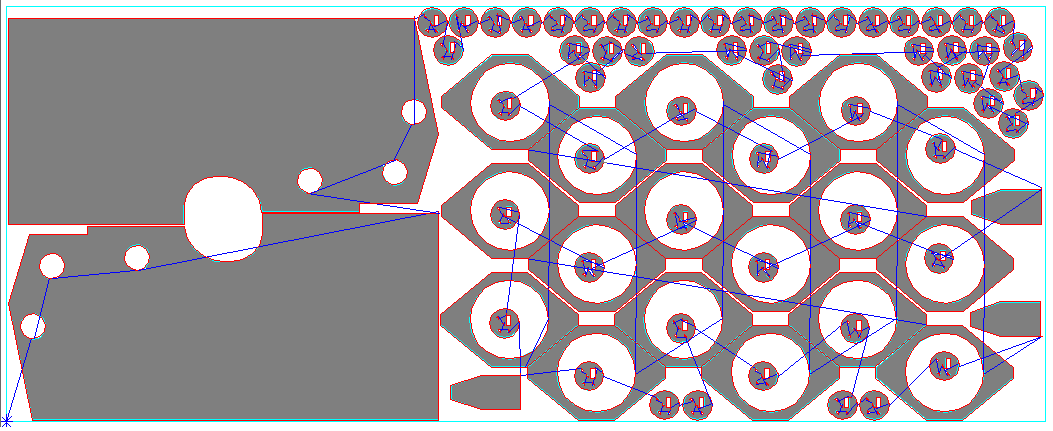
\includegraphics[width=0.9\textwidth]{spec-b.png}
  \caption{Cutting scheme example of parts using special cutting technique}
  \label{spec-b}
  \end{center}
\end{figure}

\section{Conclusion}

In this article the following results were obtained:

\bibliographystyle{splncs04}
\bibliography{tavaeva}
\nocite{*}

\end{document}
